\documentclass[10pt]{beamer}
\usepackage[utf8]{inputenc}
\usepackage[T1,T2A]{fontenc}
\usepackage[russian]{babel}
\usepackage{color}
\usepackage{calc}
\usepackage{graphicx}
\usepackage{epstopdf}
\usepackage{hyperref}
\hypersetup{unicode,colorlinks}
\usepackage{csquotes}
\usepackage{upquote}
\usepackage{cprotect}
\usetheme[progressbar=head,numbering=fraction,block=fill]{metropolis}
\usepackage{dejavu}
\usepackage{etoolbox}
\usepackage{bm}
\usepackage[ND]{prftree}
\usepackage[tableaux]{prooftrees}
\usepackage{mathtools} % for bigtimes
\usepackage{diagbox}
\usepackage{verbatimbox}
\usepackage{fitch}
\usepackage{enumitem}
%\usepackage[defaultsans]{droidsans}
%\usepackage[defaultmono]{droidmono}
%\makeatletter
%\input droid/t1fdm.fd
%\makeatother

\makeatletter
\DeclareRobustCommand*{\bfseries}{%
    \not@math@alphabet\bfseries\mathbf
    \fontseries\bfdefault\selectfont
    \boldmath
}
\makeatother

\makeatletter
\chardef\straightquote@code=\catcode`'
\chardef\backquote@code=\catcode``
\catcode`'=\active \catcode``=\active
\patchcmd{\@noligs}
{\textasciigrave}
{\fixedtextasciigrave}
{}{}
\newcommand{\fixedtextasciigrave}{%
    \makebox[.5em]{\fontencoding{TS1}\fontfamily{fvs}\selectfont\textasciigrave}% Vera Sans
}
\catcode\lq\'=\straightquote@code
\catcode\lq\`=\backquote@code
\makeatletter

\setbeamercovered{again covered={\opaqueness<1->{25}}}

\forestset{close with=\ensuremath{\bigtimes}}

\newcommand{\customframefont}[1]{
    \setbeamertemplate{itemize/enumerate body begin}{#1}
    \setbeamertemplate{itemize/enumerate subbody begin}{#1}
}

\NewEnviron{framefont}[1]{
    \customframefont{#1} % for itemize/enumerate
    {#1 % For the text outside itemize/enumerate
        \BODY
    }
    \customframefont{\normalsize}
}


\makeatletter
\DeclareRobustCommand{\rvdots}{%
    \vphantom{\int\limits^x}\smash[t]{\vdots}
}
\makeatother

\newcommand{\N}{\mathbb{N}}
\newcommand{\Z}{\mathbb{Z}}
\newcommand{\Q}{\mathbb{Q}}
\newcommand{\R}{\mathbb{R}}
\newcommand{\pow}[1]{\mathcal{P}({#1})}
\newcommand{\continuum}{\mathfrak{c}}

\author{Алексей Романов}
\subtitle{Математическая логика и теория алгоритмов}
%\logo{}
\institute{МИЭТ}
\subject{Математическая логика и теория алгоритмов}
%\setbeamercovered{transparent}
%\setbeamertemplate{navigation symbols}{}


\title{Теория множеств\\Вполне упорядоченные множества и аксиома выбора}
\date{\today}

\begin{document}
\begin{frame}[plain]
\maketitle
\end{frame}

\begin{frame}
    \frametitle{Отношения порядка}
    \begin{itemize}
        \item Напомню: бинарное отношение $\preccurlyeq$ на множестве $A$ называется \emph{отношением (частичного, нестрогого) порядка}, если оно:
        \begin{itemize}
            \item Рефлексивно: \( \forall x:A~ x \preccurlyeq x \)
            \item Антисимметрично: \( \forall x,y:A ~ x \preccurlyeq y \land y \preccurlyeq x \to x = y \)
            \item Транзитивно: \( \forall x,y,z:A ~ x \preccurlyeq y \land y \preccurlyeq z \to x \preccurlyeq z \)
        \end{itemize}
        \item Если ещё \( \forall x,y:A ~ x \preccurlyeq y \lor y \preccurlyeq x \), то это \emph{отношение линейного порядка}.
        \item Пара \((A, \preccurlyeq)\) называется \emph{частично (соотв. линейно) упорядоченным множеством}, сокращённо ЧУМ (ЛУМ).
        \item $x \prec y$, если $x \preccurlyeq y \land x \neq y$.
        \pause
        \item $x$ "--- \emph{наименьший элемент $A$}, если \(\forall y:A ~ x \preccurlyeq y\), и \emph{минимальный}, если \(\neg \exists y:A ~ y \prec x\).
        \item Для ЛУМ минимальный и наименьший одно и то же, а для ЧУМ нет.
    \end{itemize}
\end{frame}

\begin{frame}
    \frametitle{Порядковые изоморфизмы}
\begin{itemize}
    \item Биекция \(f: A \to B\) между двумя ЧУМ называется \emph{порядковым изоморфизмом}, если \( \forall x,y:A ~ x \preccurlyeq_A y \leftrightarrow f(x) \preccurlyeq_B f(y) \).
    \item В этой лекции все изоморфизмы порядковые, дальше это слово опускаем.
    \pause
    \item Если $A$ "--- ЛУМ из $n$ элементов, то оно изоморфно \(\{1,\ldots,n\}\).
    \pause
    \item Доказательство: в $A$ есть наименьший элемент. Обозначим его $a_1$ и сопоставим с $1$. $A \setminus \{a_1\}$ снова конечно и линейно упорядочено. \pause Выберем из него наименьший $a_2$ и сопоставим с $2$. И т.д.
    \pause
    \item Следствие: два равномощных конечных ЛУМ изоморфны.
    \item Для бесконечных это не так! Например, \pause \(\mathbb{N}\), \(\mathbb{Z}\) и \(\mathbb{Q}\) не изоморфны (почему?).
%    \item Как насчёт $\mathbb{N}$ и \(\mathbb{N} + \mathbb{N}\)? на семинаре
\end{itemize}
\end{frame}

\begin{frame}
    \frametitle{Фундированные и вполне упорядоченные множества}
    \begin{itemize}
        \item Вспомните \emph{принцип полной индукции} на \(\mathbb{N}\): \pause Пусть \(P(x)\) свойство натуральных чисел, и можно доказать, что если оно верно для всех \(y \prec x\), то оно верно для \(x\). Тогда оно верно для всех натуральных чисел. Формально: \( \forall x ~ (\forall y < x ~ P(y)) \to P(x)) \to \forall x ~ P(x) \)
        \pause
        \item Для каких ещё ЧУМ он выполняется?
        \item Теорема: следующие 3 утверждения равносильны для любого ЧУМ $A$:
        \begin{enumerate}
            \item В любом непустом подмножестве $A$ есть минимальный элемент.
            \item В $A$ нет бесконечных убывающих последовательностей $a_1 \succ a_2 \succ \ldots$.
            \item Принцип полной индукции для $A$.
        \end{enumerate}
        \item Такое ЧУМ называется \emph{фундированным}.
    \end{itemize}
\end{frame}

\begin{frame}
    \frametitle{Множество фундировано $\Leftrightarrow$ нет бесконечных убывающих последовательностей}
    \begin{itemize}
        \item $1 \Rightarrow 2$: Если $a_1 \succ a_2 \succ \ldots$ "--- бесконечная убывающая последовательность, то \pause \(\{a_1,a_2,\ldots\}\) "--- непустое множество без минимального элемента.
        \pause
        \item $2 \Rightarrow 1$: Если $B$ "--- непустое подмножество $A$ без минимального элемента, то \pause возьмём его произвольный элемент и обозначим $a_1$. \pause Так как он не минимальный, то есть $a_2 \prec a_1$. \pause Аналогично есть $a_3 \prec a_2$\ldots
    \end{itemize}
\end{frame}

\begin{frame}
    \frametitle{Множество фундировано $\Leftrightarrow$  принцип полной \\ индукции}
    \begin{itemize}
        \item $1 \Rightarrow 3$: Пусть $P(x)$ "--- свойство на $A$, для которого верно \( \forall x ~ (\forall y \prec x ~ P(y)) \to P(x) \), но не \( \forall x ~ P(x) \). Рассмотрим \(B = \{x:A \mid \neg P(x)\} \). Оно непусто. Так как $A$ фундировано, в $B$ есть минимальный элемент $b$. Но тогда \pause $\forall x : A ~ x \prec b \Rightarrow x \notin B \Rightarrow P(x)$ и по предположению ППИ $P(b)$, то есть $b \notin B$. Противоречие!
        \pause
        \item $3 \Rightarrow 1$: Если $B$ "--- подмножество $A$ без минимального элемента, то рассмотрим \( P(x) \Leftrightarrow x \notin B \). Имеем \((\forall y \prec x ~ P(y)) \Rightarrow (\forall y \prec x ~ y \notin B) \Rightarrow x \notin B \) (иначе $x$ минимальный в $B$) $\Rightarrow P(x)$\pause. По ППИ \( \forall x ~ P(x) \Rightarrow \forall x ~ x \notin B \Rightarrow B \) пусто.
    \end{itemize}
\end{frame}

\begin{frame}
    \frametitle{Операции над ЧУМ}
    \begin{itemize}
        \item Любое подмножество $B$ ЧУМ $A$ имеет \emph{индуцированный порядок}. 
        \item Если $A$ и $B$ непересекающиеся ЧУМ, то $A+B$ это $A \cup B$ с порядком \[ x \prec_{A+B} y \Leftrightarrow (x,y \in A \land x \prec_A y) \lor (x,y \in B \land x \prec_B y) \lor (x \in A \land y \in B) \]
        \item Порядок на $A \times B$ лексикографический, то есть 
        \[ (a_1, b_1) \prec_{A \times B} (a_2, b_2) \Leftrightarrow a_1 \prec_A a_2 \lor (a_1 = a_2 \land b_1 \prec_B b_2) \]
        \item Если $A$ и $B$ фундированы и/или линейны, то $A+B$ и $A \times B$ тоже. Доказательство как упражнение.
    \end{itemize}
\end{frame}

\begin{frame}
    \frametitle{Вполне упорядоченные множества}
    \begin{itemize}
        \item Фундированное ЛУМ называется \emph{вполне упорядоченным}.
        \item Некоторые простые свойства:
        \item Любое непустое ВУМ имеет наименьший элемент.
        \item Если элемент $x$ ВУМ не наибольший, то есть непосредственно следующий за ним $S(x)$ (или $x+1$).
        \item У не-наименьшего элемента ВУМ может не быть непосредственно предыдущего. Такой элемент называется \emph{предельным}.
        \item Любое ограниченное сверху подмножество ВУМ имеет супремум (точную верхнюю грань).
        \item Любое подмножество ВУМ само вполне упорядочено.
    \end{itemize}
\end{frame}

\begin{frame}
    \frametitle{Начальные отрезки}
    \begin{itemize}
        \item $B \subseteq A$ "--- \emph{начальный отрезок $A$}, если любой элемент $B$ меньше любого элемента $A \setminus B$. Равносильно: все элементы, меньшие какого-то элемента $B$, лежат в $B$.
        \item Это определение имеет смысл для любого ЛУМ, но нам интересно только для ВУМ.
        \item В том числе $\varnothing$ и $A$ "--- начальные отрезки $A$. 
        \item Если все элементы множества $D$ "--- начальные отрезки ВУМ $A$, то $\bigcup D$ тоже начальный отрезок $A$.
        \item $B$ "--- собственный начальный отрезок ВУМ $A$ (т.е. $B \neq A$) $\Leftrightarrow \exists x:A ~ B = \{y:A \mid y \prec x\}$. Обозначим $\{y:A \mid y \prec x\}$ как $A_{\prec x}$.
        \item Если $B$ и $C$ начальные отрезки ВУМ $A$, то $B \subseteq C \lor C \subseteq B$.
    \end{itemize}
\end{frame}

\begin{frame}
    \frametitle{Теоремы о сравнении ВУМ}
    \begin{itemize}
        \item Теорема: пусть $A$ и $B$ ВУМ. Тогда либо $A$ изоморфно какому-то начальному отрезку $B$ (возможно, самому $B$), либо наоборот.
        \item Теорема: ВУМ $A$ никогда не изоморфно своему собственному начальному отрезку $B$.
        \item Доказательства: сейчас давать не буду, можно найти в книге Шеня-Верещагина.
        \item Следствие: любые ВУМ $A$ и $B$ либо изоморфны, либо ровно одно из них изоморфно собственному начальному отрезку другого.
    \end{itemize}
\end{frame}

\begin{frame}
    \frametitle{Аксиома выбора}
    \begin{itemize}
        \item Пусть $A$ произвольное множество непустых множеств. Тогда существует такая \emph{функция выбора} $ch_A: A \to \bigcup A$, что $\forall B:A~ch_A(B) \in B$.
        \item Можно сформулировать то же для индексированных семейств непустых множеств: если $A = \langle A_i \rangle_{i : I}$, то $ch_A: I \to \bigcup_{i : I} A_i,~\forall i:I~ch_A(i) \in A_i$.
        \item Эта аксиома не входит в исходную теорию Цермело--Френкеля $ZF$, её добавление даёт $ZFC$, стандартное основание математики.
        \item Заметьте, что \enquote{дано непустое множество, выберем в нём элемент} не требует аксиомы выбора.
        \item То же и для конечных $A$ (и $I$) в определении выше.
        \item Аксиома выбора нужна, чтобы сделать одновременно бесконечно много таких выборов и зафиксировать их.
    \end{itemize}
\end{frame}

\begin{frame}
    \frametitle{Лемма Цорна}
    \begin{itemize}
        \item \emph{Цепь} в ЧУМ "--- такое подмножество, любые два элемента которого сравнимы.
        \item Если в ЧУМ $A$ любая цепь $B$ имеет верхнюю грань ($\exists x : A ~ \forall y : B ~ y \preccurlyeq x$), то в $A$ есть максимальный элемент.
        \item (Вспомните разницу между максимальным и наибольшим!)
        \item Доказательство тоже в учебнике.
        \pause
        \item Можно немного усилить и показать, что для любого $x$ в таком $A$ есть максимальный $y$ такой, что $y \succcurlyeq x$.
        \pause
        \item[]
        \item Типичное применение леммы Цорна: в любом линейном пространстве $L$ есть базис.
        \pause
        \item Для доказательства возьмём $A = \{S \subset L \mid S$ линейно независимо$\}$ с порядком по включению.
        \item Верхняя грань любой цепи в нём "--- объединение.
        \item Максимальный элемент и будет базисом.
    \end{itemize}
\end{frame}

\begin{frame}
    \frametitle{Теорема Цермело}
    \begin{itemize}
        \item На любом множестве $A$ можно задать отношение вполне порядка $\preccurlyeq$.
        \item Идея доказательства (остаётся доказать 2 и 4):
        \begin{enumerate}
            \item Возьмём множество $WO_A$ пар $(B, \preccurlyeq_B)$, где $B \subseteq A, \preccurlyeq_B$ "--- вполне порядок на $B$. Отношение \enquote{быть начальным отрезком}~"--- частичный порядок на нём.
            \item Для любой цепи в этом порядке объединение множеств будет верхней гранью.
            \item По лемме Цорна есть максимальное $(B^*, \preccurlyeq_{B^*}) \in WO_A$.
            \item Если $B^* \neq A$, то оно не будет максимальным.
            \item Значит, $B^* = A$, и $\preccurlyeq_{B^*}$ "--- искомый вполне порядок на $A$.
        \end{enumerate}
        \item При этом ни на каком несчётном множестве задать такое отношение порядка явно формулой $ZFC$ невозможно.
    \end{itemize}
\end{frame}

\begin{frame}
    \frametitle{Эквивалентные формы аксиомы выбора}
    \begin{itemize}
        \item Аксиома выбора, теорема Цермело и лемма Цорна эквивалентны.
        \item Доказательство аксиомы выбора из теоремы Цермело просто: введём вполне порядок $\prec$ на $\bigcup A$ и для любого $B \in A$ выберем из $B$ \pause $\min B$ по $\prec$.
        \item Шутка Джерри Бона: \enquote{АВ очевидно истинна, ТЦ очевидно ложна, а кто может сказать про ЛЦ?}.
        \pause
        \item Другие эквивалентные им утверждения:
        \begin{enumerate}
            \item Декартово произведение непустого множества непустых множеств непусто (его элементы и есть функции выбора на этом множестве).
            \item У каждого наложения есть правая обратная функция.
            \item В любом ЧУМ существует максимальная цепь (принцип максимума Хаусдорфа).
            \item Любое бесконечное $A$ равномощно $A \times A$.
            \item Любые два множества сравнимы по мощности.
            \item В любом линейном пространстве есть базис.
        \end{enumerate}
    \end{itemize}
\end{frame}

\begin{frame}
    \frametitle{Следствия аксиомы выбора}
    \begin{itemize}
        \item Парадокс Банаха--Тарского (также известный как парадокс удвоения шара) следует из аксиомы выбора.
        \item Как и вообще существование неизмеримых множеств.
        \item Если множество $A$ бесконечно, то существует вложение $\N \to A$.
        \item Если бесконечные $A$ и $B$ равномощны и не пересекаются, то $A \cup B \sim A$.
        \item Если в векторном пространстве нет конечного базиса, то в нём есть бесконечное линейно независимое множество векторов.
    \end{itemize}
\end{frame}

\begin{frame}
    \frametitle{Слабые формы аксиомы выбора}
    \begin{itemize}
        \item Аксиома счётного выбора $AC_\omega$ это аксиома выбора для счётных множеств $A$. С индексами: если дана последовательность непустых множеств $\langle A_n \rangle_{n : \N}$, то можно выбрать по элементу из каждого: существует $f:\pause \N \to \bigcup_{n \in \N} A_n, \pause\forall n~f(n) \in A_n$.
        \begin{itemize}
            \item Пример следствия (но не эквивалентно!): объединение счётного множества счётных множеств счётно.
        \end{itemize}
        \pause
        \item Аксиома зависимого выбора $DC$: если $A$ непустое множество, $R$ бинарное отношение на нём и $\forall x:A~\exists y:A~xRy$, то существует бесконечная последовательность $x_n:A$ такая, что $\forall n:\N~x_nRx_{n+1}$.
        \begin{itemize}
            \item Это эквивалентно лемме Цорна для конечных цепей: если в ЧУМ все цепи конечны, то там есть максимальный элемент.
        \end{itemize}
        \pause
        \item $AC \Rightarrow DC \Rightarrow AC_\omega$.
    \end{itemize}
\end{frame}

\begin{frame}
    \frametitle{Ординалы}
    \begin{itemize}
        \item \emph{Ординалы} можно определить по аналогии с мощностями: это классы эквивалентности ВУМ по отношению изоморфности (\emph{порядковые типы}).
        \item То есть у любого ВУМ есть ординал, и ординалы изоморфных ВУМ равны.
        \item Но есть более удобное индуктивное определение:
        \begin{itemize}
            \item $0 = \varnothing$ это ординал.
            \item Если $\alpha$ ординал, то $\alpha + 1 = S(\alpha) = \alpha \cup \{\alpha\}$ тоже ординал.
            \item Если $A$ множество, все элементы которого ординалы, то $\sup A = \bigcup A$ тоже ординал.
        \end{itemize}
        \item \emph{Предельный ординал} "--- такой, который не $0$ и не следует ни за каким ординалом.
        \item То есть его можно получить только как супремум.
        \item С помощью аксиомы выбора, можно доказать, что любое ВУМ изоморфно одному из таких ординалов.
        \item Класс всех ординалов обозначается $Ord$.
    \end{itemize}
\end{frame}

\begin{frame}
    \frametitle{Структура счётных ординалов (до $\omega^\omega$)}
    \begin{itemize}
        \item $0 = \varnothing$.
        \item $1 = S(0) = 0 \cup \{0\} = \{0\}$. \pause
        \item $2 = S(1) = \{0,1\}$.
        \item \ldots \pause
        \item $\omega = \sup \{0,1,2,\ldots\} = 0 \cup 1 \cup 2 \cup \ldots = \pause \{0,1,2,\ldots\}$. \pause
        \item $\omega + 1 = \omega \cup \{\omega\} = \{0,1,2,\ldots,\omega\}$.
        \item $\omega + 2 = \{0,1,2,\ldots,\omega,\omega + 1\}$.
        \item \ldots \pause
        \item $\omega \cdot 2 = \sup \{\omega, \omega + 1, \omega + 2, \ldots\} = \pause \{0,1,2,\ldots, \omega, \omega + 1, \omega + 2, \ldots\}$.
        \item $\omega \cdot 2 + 1 = \{0,1,2,\ldots, \omega, \omega + 1, \omega + 2, \ldots, \omega \cdot 2\}$.
        \item \ldots \pause
        \item $\omega^2 = \omega \cdot \omega = \sup \{\omega, \omega \cdot 2, \omega \cdot 3, \ldots\} = \pause \{0,1,2,\ldots, \omega, \omega + 1, \omega + 2, \ldots, \omega \cdot 2, \omega \cdot 2 + 1, \ldots\}$.
        \item \ldots
    \end{itemize}
\end{frame}

\begin{frame}
    \frametitle{Структура счётных ординалов (до $\omega^\omega$)}
    \centering
    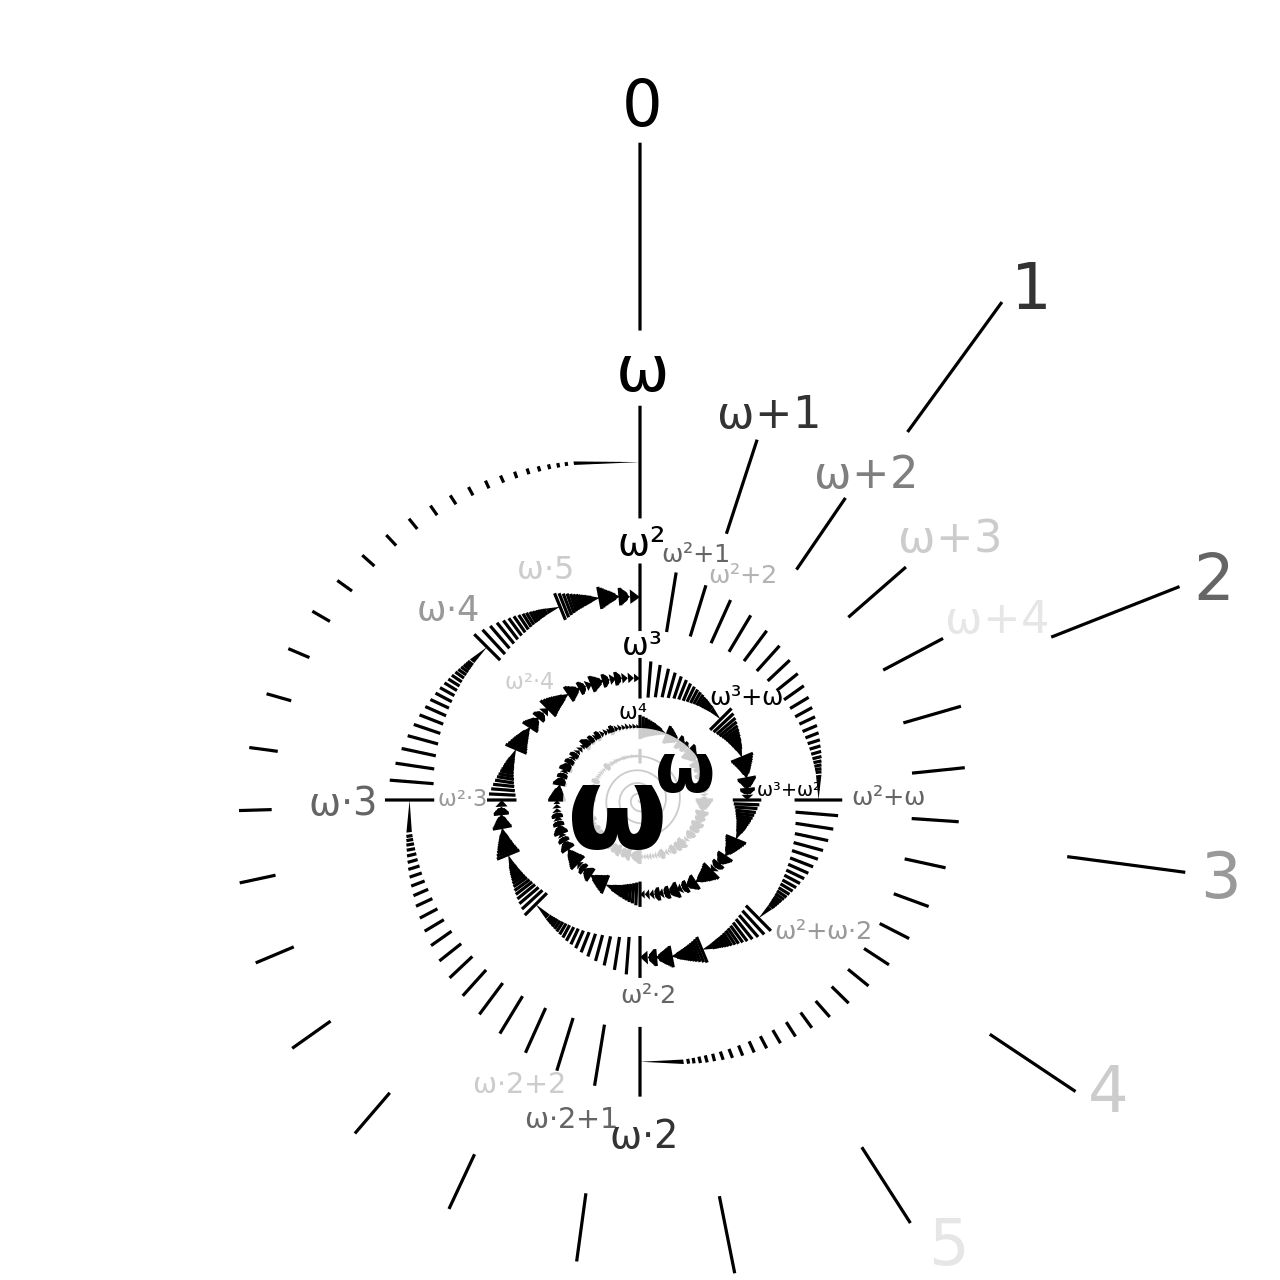
\includegraphics[width=\textwidth,height=0.9\textheight,keepaspectratio]{Omega-exp-omega.svg.png}
\end{frame}

\begin{frame}
    \frametitle{Порядок на ординалах}
    \begin{itemize}
        \item $\alpha < \beta \Leftrightarrow \alpha \in \beta \Leftrightarrow \alpha \subsetneq \beta$.
        \item Каждый ординал равен множеству всех ординалов, меньших него: $\alpha = \{\beta | \beta < \alpha\}$.
        \item Легко доказать, что $\leq$ действительно отношение порядка: рефлексивно, транзитивно и антисимметрично. И линейно.
        \item Более того, ординалы вполне упорядочены: в любом классе (не только множестве) ординалов есть наименьший.
        \item Теперь можно проверить, что если $A$ множество ординалов, то $\bigcup A$ это действительно $\sup A$, то есть наименьшая верхняя грань.
    \end{itemize}
\end{frame}

\begin{frame}
    \frametitle{Парадокс Бурали-Форти}
    \begin{itemize}
        \item Ограничение \enquote{если $A$ множество} в определении ординала-супремума существенное: множества всех ординалов не существует.
        \item Допустим, что $Ord$ множество. Тогда $O = \sup Ord + 1$ ординал, но это не элемент $Ord$. Почему? \pause
        \item Например, потому что он больше всех элементов $Ord$. \pause
        \item Но тогда получится, что $Ord$ содержит не все ординалы. Пришли к противоречию!
    \end{itemize}
\end{frame}

\begin{frame}
    \frametitle{Арифметика над ординалами}
    \begin{itemize}
        \item Операции над ординалами определяются по рекурсии:
        \begin{itemize}
            \item $\alpha + 0 = \alpha$.
            \item $\alpha + S(\beta) = S(\alpha + \beta)$.
            \item $\alpha + \sup A = \sup \{\alpha + \beta | \beta \in A\}$.
        \end{itemize}
        \item
        \begin{itemize}
            \item $\alpha \cdot 0 = 0$.
            \item $\alpha \cdot S(\beta) = \alpha \cdot \beta + \alpha$.
            \item $\alpha \cdot \sup A = \sup \{\alpha \cdot \beta | \beta \in A\}$.
        \end{itemize}
        \item
        \begin{itemize}
            \item $\alpha^0 = 1$.
            \item $\alpha^{S(\beta)} = \alpha^\beta \cdot \alpha$.
            \item $\alpha^{\sup A} = \sup \{\alpha^\beta | \beta \in A\}$.
        \end{itemize}
    \end{itemize}
\end{frame}

\begin{frame}
    \frametitle{Арифметика над ординалами}
    \begin{itemize}
        \item Например, $1 + \omega = 1 + \sup \{0, 1, 2, \ldots\} \pause = \sup \{1, 2, 3, \ldots\} = \bigcup \{1, 2, 3, \ldots\} = \{0, 1, \ldots\} = \omega$.
        \item Многие привычные свойства арифметики для ординалов сохраняются, но как видим, не все.
    \end{itemize}
\end{frame}

\begin{frame}
    \frametitle{Кардиналы}
    \begin{itemize}
        \item С помощью ординалов мы можем дать окончательное определение $|A|$ так, чтобы она была множеством.
        \pause
        \item По теореме Цермело $A$ можно вполне упорядочить. То есть $A$ биективно какому-то ординалу.
        \item Тогда класс $\{\alpha | \alpha:Ord, A \sim \alpha\}$ непуст и имеет \pause минимум. Этот минимум и есть $|A|$.
        \item Видно ли, что если $A \sim B$, то $|A| = |B|$, как и требуется?
        \item Все значения $|A|$ (то есть минимальные ординалы какой-то мощности) называются кардиналами.
        \pause
        \item Они сами тоже вполне упорядочены.
        \item $\aleph_0$ это наименьший бесконечный кардинал, $\aleph_1$ это наименьший кардинал $>\aleph_0$, и так далее.
        \item Индексы алефов "--- ординалы, то есть для любого ординала $\alpha$ определено $\aleph_\alpha$.
    \end{itemize}
\end{frame}

\newlength{\geqwidth}
\settowidth{\geqwidth}{$\geq$}

\begin{frame}
    \frametitle{Континуум-гипотеза}
    \begin{itemize}
        \item Мы знаем, что $\continuum > \aleph_0$, то есть $\continuum \alt<1>{\mathmakebox[\geqwidth]{?}}{\geq} \aleph_1$.
        \pause \pause % именно 2 паузы
        \item Естественно предположить, что $\continuum = \aleph_1$, то есть нет промежуточных мощностей между $\aleph_0$ и $\continuum$.
        \item Это называется \emph{континуум-гипотезой} $CH$.
        \pause
        \item Оказывается, что в $ZFC$ это нельзя ни доказать, ни опровергнуть: есть модели $ZFC$, в которых $\continuum = \aleph_1$, а есть такие, в которых $\continuum = \aleph_2$, $\aleph_\omega$ и т.д.
        \item То же самое верно для \emph{обобщённой континуум-гипотезы} $GCH$: $2^{\aleph_\alpha} = \aleph_{\alpha+1}$ для всех $\alpha$.
        \pause
        \item Проще найти модель, в которой $GCH$ верна: это \emph{конструктивный универсум} $L$, состоящий из таких множеств, которые можно определить с помощью формул $ZFC$, в которых используются только ранее сконструированные множества.
    \end{itemize}
\end{frame}

\begin{frame}
    \frametitle{Трансфинитная иерархия всех множеств и \\ конструктивная иерархия}
    \begin{itemize}
        \item Универсум всех множеств $V$ можно разбить на ранги:
        \begin{itemize}
            \item $V_0 = \varnothing$.
            \item $V_{\alpha+1} = \pow{V_\alpha}$ "--- множество всех подмножеств $V_\alpha$. Оно будет включать $V_\alpha$.
            \item Если $\lambda$ предельный ординал, то $V_\lambda = \bigcup_{\alpha < \lambda} V_\alpha$.
            \item $V = \bigcup_{\alpha : Ord} V_\alpha$.
        \end{itemize}
        \item При этом можно записать формулу $ZFC$ $rk(X, \alpha)$, которая означает $X \in V_\alpha$.
        \item И можно доказать $\forall X \exists \alpha~ord(\alpha) \land rk(X, \alpha)$ (то есть любое $X$ имеет какой-то ранг $\alpha$ и является элементом $V$).
        \pause
        \item Теперь определение $L$ отличается только в одном:
        \begin{itemize}
            \item $L_{\alpha+1}$ это множество не всех подмножеств $L_\alpha$, а тех, которые можно определить формулой сигнатуры $ZFC$ с параметрами из $L_\alpha$ и только с кванторами по $L_\alpha$.
            \item Вместо понятия определимости можно использовать фиксированный набор операций над элементами $L_\alpha$.
        \end{itemize}
    \end{itemize}
\end{frame}

\end{document}
